%%%%%%%% ICML 2023 EXAMPLE LATEX SUBMISSION FILE %%%%%%%%%%%%%%%%%

\documentclass{article}

% Recommended, but optional, packages for figures and better typesetting:
\usepackage{microtype}
\usepackage{graphicx}
\usepackage{subfigure}
\usepackage{booktabs} % for professional tables
\usepackage{animate}


\usepackage{tikz}
% Corporate Design of the University of Tübingen
% Primary Colors
\definecolor{TUred}{RGB}{165,30,55}
\definecolor{TUgold}{RGB}{180,160,105}
\definecolor{TUdark}{RGB}{50,65,75}
\definecolor{TUgray}{RGB}{175,179,183}

% Secondary Colors
\definecolor{TUdarkblue}{RGB}{65,90,140}
\definecolor{TUblue}{RGB}{0,105,170}
\definecolor{TUlightblue}{RGB}{80,170,200}
\definecolor{TUlightgreen}{RGB}{130,185,160}
\definecolor{TUgreen}{RGB}{125,165,75}
\definecolor{TUdarkgreen}{RGB}{50,110,30}
\definecolor{TUocre}{RGB}{200,80,60}
\definecolor{TUviolet}{RGB}{175,110,150}
\definecolor{TUmauve}{RGB}{180,160,150}
\definecolor{TUbeige}{RGB}{215,180,105}
\definecolor{TUorange}{RGB}{210,150,0}
\definecolor{TUbrown}{RGB}{145,105,70}

% hyperref makes hyperlinks in the resulting PDF.
% If your build breaks (sometimes temporarily if a hyperlink spans a page)
% please comment out the following usepackage line and replace
% \usepackage{icml2023} with \usepackage[nohyperref]{icml2023} above.
\usepackage{hyperref}


% Attempt to make hyperref and algorithmic work together better:
\newcommand{\theHalgorithm}{\arabic{algorithm}}

\usepackage[accepted]{icml2023}

% For theorems and such
\usepackage{amsmath}
\usepackage{amssymb}
\usepackage{mathtools}
\usepackage{amsthm}

% if you use cleveref..
\usepackage[capitalize,noabbrev]{cleveref}

%%%%%%%%%%%%%%%%%%%%%%%%%%%%%%%%
% THEOREMS
%%%%%%%%%%%%%%%%%%%%%%%%%%%%%%%%
\theoremstyle{plain}
\newtheorem{theorem}{Theorem}[section]
\newtheorem{proposition}[theorem]{Proposition}
\newtheorem{lemma}[theorem]{Lemma}
\newtheorem{corollary}[theorem]{Corollary}
\theoremstyle{definition}
\newtheorem{definition}[theorem]{Definition}
\newtheorem{assumption}[theorem]{Assumption}
\theoremstyle{remark}
\newtheorem{remark}[theorem]{Remark}

% Todonotes is useful during development; simply uncomment the next line
%    and comment out the line below the next line to turn off comments
%\usepackage[disable,textsize=tiny]{todonotes}
\usepackage[textsize=tiny]{todonotes}


% The \icmltitle you define below is probably too long as a header.
% Therefore, a short form for the running title is supplied here:
\icmltitlerunning{Project Report Template for Data Literacy 2023/24}

\begin{document}

\twocolumn[
\icmltitle{Beyond the Beer Tent: An Analysis of Oktoberfest's Yearly Visitor,\\ Consumption, and Price Trends)}

% It is OKAY to include author information, even for blind
% submissions: the style file will automatically remove it for you
% unless you've provided the [accepted] option to the icml2023
% package.

% List of affiliations: The first argument should be a (short)
% identifier you will use later to specify author affiliations
% Academic affiliations should list Department, University, City, Region, Country
% Industry affiliations should list Company, City, Region, Country

% You can specify symbols, otherwise they are numbered in order.
% Ideally, you should not use this facility. Affiliations will be numbered
% in order of appearance and this is the preferred way.
\icmlsetsymbol{equal}{*}

\begin{icmlauthorlist}
\icmlauthor{Jana Hoffmann}{equal,first}
\icmlauthor{Julia Graf}{equal,second}
\icmlauthor{Jessie Midgley}{equal,third}
\icmlauthor{Tithi Rakshit}{equal,fourth}
\end{icmlauthorlist}

% fill in your matrikelnummer, email address, degree, for each group member
\icmlaffiliation{first}{Matrikelnummer 5760486, jana2.hoffmann@student.uni-tuebingen.de, MSc Bioinformatics}
\icmlaffiliation{second}{Matrikelnummer 5656882, jul.graf@student.uni-tuebingen.de, MSc Bioinformatics}
\icmlaffiliation{third}{Matrikelnummer 6620875, jessie.midgley@student.uni-tuebingen.de, MSc Bioinformatics}
\icmlaffiliation{fourth}{Matrikelnummer 6635972, tithi.rakshit@student.uni-tuebingen.de, MSc Quantitative Data Science}

% You may provide any keywords that you
% find helpful for describing your paper; these are used to populate
% the "keywords" metadata in the PDF but will not be shown in the document
\icmlkeywords{Machine Learning, ICML}

\vskip 0.3in
]

% this must go after the closing bracket ] following \twocolumn[ ...

% This command actually creates the footnote in the first column
% listing the affiliations and the copyright notice.
% The command takes one argument, which is text to display at the start of the footnote.
% The \icmlEqualContribution command is standard text for equal contribution.
% Remove it (just {}) if you do not need this facility.

%\printAffiliationsAndNotice{}  % leave blank if no need to mention equal contribution
\printAffiliationsAndNotice{\icmlEqualContribution} % otherwise use the standard text.

\begin{abstract}
Analyzing visitor statistics, precipitation data, and consumption trends over the last 38 years, we explore the evolution of the Oktoberfest and its impact on tourism in Munich and surrounding areas. Our findings highlight fluctuations in visitor numbers, and reveal insights into the festival's resilience in the face of external factors such as weather. Additionally, we investigate the influx of tourists to Upper Bavaria during Oktoberfest and observe deviations in guest arrivals compared to expectations. Furthermore, we analyze trends in beer and chicken consumption and prices, noting a positive correlation between beer price and consumption. We employ regression models to predict beer and chicken prices for 2023, demonstrating varying degrees of accuracy between linear and Gaussian process regression models.
\end{abstract}

\section{Introduction}\label{sec:intro}
The Oktoberfest, held in Munich, Germany, is one of the world's most renowned folk festivals, attracting millions annually. In this paper, we analyze nearly four decades of Oktoberfest data, spanning from 1985 to 2023, to uncover insights into its evolution and various influencing factors. Understanding the dynamics of this iconic event is not only of cultural significance but also holds economic and societal implications. \\
 This paper is structured as follows: \Cref{sec:methods} outlines our data sources and analytical methods. \Cref{sec:results} presents our findings, elucidating key trends and correlations observed within the Oktoberfest dataset, and \Cref{sec:conclusion} discusses the implications of our findings and offers insights into future festivals.\\
Our discoveries shed light on the dynamics of Oktoberfest and its wider implications, providing valuable information that could be useful in the future planning of this festival.

\section{Data and Methods}\label{sec:methods}
The annual Oktoberfest data from 1985 to 2022 was retrieved from the Open Data Portal of the Statistical Office Munich~\citep{5}. This dataset contains the yearly festival duration, visitor numbers, as well as consumption and prices for beer and roast chicken. Additional data for 2023 was retrieved from the State Capital Munich Portal~\citep{6,7}. \\
We examine the evolution of visitor numbers over the years and use four additional datasets to investigate how these are influenced by precipitation. Weather datasets were retrieved from the Open Data Server of the German Meteorological Service (DWD) and contain data from the weather stations ``München-Stadt" and ``München (Bavariaring)". Two of the datasets contain the daily precipitation in millimeters, with one spanning from 1954 to 2022, and the other from 2022 to 2024~\citep{3,4}. The remaining two datasets contain the hourly precipitation in millimeters, in ranges from 1997 to 2022, and from 2022 to 2024~\citep{1,2}. We use the Pearson correlation coefficient (PCC) to investigate the correlation between the average number of daily visitors and the average daily precipitation during each Oktoberfest, and also constrain daily precipitation between 10am and 10pm. The PCC ranges from -1 to 1, where a high absolute value indicates a strong correlation between two variables~\cite{thonield}.\\
To investigate the impact of Oktoberfest on visitor numbers in the surrounding districts of Munich, we obtained monthly visitor numbers for February, March, April, August, September, and October from 2006 to 2023 for all districts in Bavaria from the GENESIS-Online database of the Bavarian State Office for Statistics~\citep{table_GENESIS}. The visitor numbers are categorized into overnight stays and arrivals and are listed for both domestic and foreign visitors.\\
To generate a heat map of the areas that benefit the most from Oktoberfest in terms of increased visitor numbers, a methodology for calculating the number of visitors to a district who also attend the festival must be established. One possible approach is to calculate the average number of visitors for the preceding month (August) and the following month (October) to estimate the expected number of visitors without the influence of the Oktoberfest. The expected number can then be subtracted from the actual number of visitors to determine the number of visitors to the Oktoberfest. The final heat map displays the percentage deviation between the expected and actual number of visitors for the individual districts in Upper Bavaria. This correction accounts for the varying size and popularity of the districts.\\
To demonstrate the validity of the method, we applied it to three consecutive months (February, March, and April), assuming similar visitor numbers as no special events took place during these months. If this assumption is correct, our method should accurately estimate the number of visitors in March by using the average number of visitors in February and April. Validation works with any three consecutive months, as long as they are not expected to have an unusually high or low number of visitors, such as during Christmas markets or similar events.\\
We investigate visitor, price, and consumption trends over the years, and use the PCC to explore the correlation between beer price and per capita beer consumption. To adjust for inflation over time, beer prices are also divided by the Consumer Price Index (CPI) which measures the monthly average price development of goods and services purchased by German households. The CPI data was collected from the Federal Statistical Office of Germany (Destatis)~\citep{10}.\\
We utilized a Linear regression model to predict the price for the year 2023, and subsequently, compared it with the empirically observed price for the same year. To achieve an optimal fit, we assessed polynomial degrees ranging from one to ten. Additionally, we explored Gaussian process regression using the Radial Basis Function (RBF) and DotProduct kernels to estimate the price with a probabilistic approach. This same methodology was applied for forecasting the chicken price for the year 2023.

% This is the template for a figure from the original ICML submission pack. In lecture 10 we will discuss plotting in detail.
% Refer to this lecture on how to include figures in this text.
%
% \begin{figure}[ht]
% \vskip 0.2in
% \begin{center}
% \centerline{\includegraphics[width=\columnwidth]{icml_numpapers}}
% \caption{Historical locations and number of accepted papers for International
% Machine Learning Conferences (ICML 1993 -- ICML 2008) and International
% Workshops on Machine Learning (ML 1988 -- ML 1992). At the time this figure was
% produced, the number of accepted papers for ICML 2008 was unknown and instead
% estimated.}
% \label{icml-historical}
% \end{center}
% \vskip -0.2in
% \end{figure}

\section{Results}\label{sec:results}
\subsection*{3.1 Visitor trend over the years}
From the first Oktoberfest in 1985 until the most recent one in 2023, we observe a considerable fluctuation in yearly visitor numbers (Figure~\ref{figure_visitors}). We also observe a dramatic drop in visitor numbers, from 6.9 million visitors in the year 2000 to only 5.5 million in 2001. The Oktoberfest was cancelled in 2020 and 2021 due to the COVID-19 pandemic, and a new record number of 7.2 million visitors was set in 2023. To gain insight into a potential cause of this fluctuation, we investigate the influence of weather on visitor numbers.
\begin{figure}[ht]% this figure made with
  % plt.rcParams.update(bundles.icml2022(column="half”,usetex=False))
  % fig,ax = plt.subplots(nrows=1, ncols=1)
  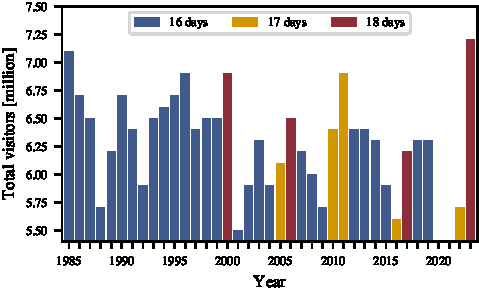
\includegraphics{fig/totalvisitors.pdf}
  \caption{The number of visitors to the Oktoberfest from 1985 to 2023. Bars are coloured depending on the duration of the festival that year.}
  \label{figure_visitors}
\end{figure}

\subsection*{3.2 Influence of precipitation on visitor numbers}
The PCC for the mean daily visitors and the mean daily precipitation each year is -0.1913. The negative correlation indicates that visitor numbers decrease as precipitation increases. Since the absolute value of the PCC is low, the correlation between the variables is weak. Since mean daily precipitation includes hours outside of festival visiting hours, we also investigate whether precipitation at daytime has a stronger correlation with visitor numbers (Figure~\ref{figure_precipitation}). We therefore considered precipitation only between 10am and 10pm, and found a PCC of -0.2276, indicating a slightly stronger negative correlation.
\begin{figure}[ht]% this figure made with
  % plt.rcParams.update(bundles.icml2022(column="half”,usetex=False))
  % fig,ax = plt.subplots(nrows=1, ncols=1)
  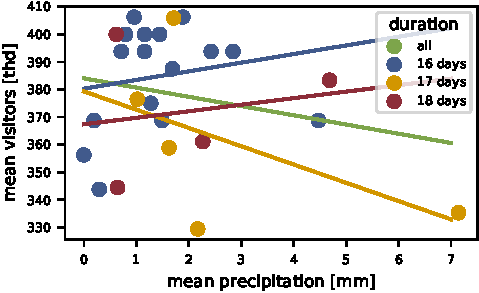
\includegraphics{fig/totalprecipitation.pdf}
  \caption{The mean daily visitors as a function of the mean daily precipitation between 10am and 10pm during the Oktoberfest each year. The green line is the linear regression line of all data points. The dots are coloured depending on the duration of the corresponding festival.}
  \label{figure_precipitation}
\end{figure}

\subsection*{3.3 Tourists to Upper Bavaria during Oktoberfest}
\begin{figure*}[ht] % this figure made with
% plt.rcParams.update(bundles.icml2022(column=”full”, nrows=1, ncols=2, usetex=False)))
% fig,ax = plt.subplots(nrows=1, ncols=2)
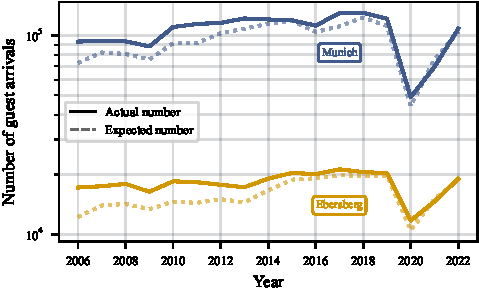
\includegraphics{fig/actual_vs_expected_arrivals.pdf} % note no [width=\textwidth] needed
\caption{Expected and actual number of guest arrivals in the month of September in the districts of Munich and Ebersberg from 2006 to 2023.}
\label{fig:exp_vs_actual_arrivals}
\end{figure*}
The Oktoberfest evidently boosts the number of visitors to Munich when it takes place in September (Figure~\ref{fig:exp_vs_actual_arrivals}). In the nearby districts around Munich (such as Ebersberg), there are smaller but still noticeable deviations between the expected and actual number of guest arrivals. Importantly, the number of guest arrivals consistently surpasses expectations, indicating the impact of Oktoberfest in these areas.
\begin{figure}[ht]
  \centering
  \animategraphics[autoplay,loop,width=1.0\linewidth]{0.5}{fig/gif_images/visitors_heatmap_}{2006}{2022}
  \caption{Percentage change between the expected and observed number of tourists in September for the individual counties of Upper Bavaria from 2006 to 2022. The areas in darker purple are those where the number of visitors has been higher than expected.}
  \label{fig:heatmap}
\end{figure}
This information can be neatly presented using a heat map to show how the number of visitors in different counties around Munich is affected by the Oktoberfest (Figure~\ref{fig:heatmap}).\textbf{}

\subsection*{3.4 Price and consumption trends}
We see an almost linear increase in beer price over the years (Figure~\ref{fig:beer_consumption}). The per capita consumption also shows an overall increase, but fluctuates over the years. We observe a low per capita beer consumption in 2023, likely due to to the record number of visitors that year. The correlation plot shows that beer consumption continues to increase, despite rising beer prices. This strong positive relationship between beer price and consumption is confirmed by the PCC of 0.8452. Adjusting beer prices by the CPI (and excluding 2023 outlier) slightly increases the correlation between beer price and consumption from 0.9473 to 0.9548. For roast chicken, a PCC coefficient of -0.8679 shows a strong negative correlation between price and consumption.
\begin{figure*}[ht] % this figure made with
% plt.rcParams.update(bundles.icml2022(column=”full”, nrows=1, ncols=2, usetex=False)))
% fig,ax = plt.subplots(2)
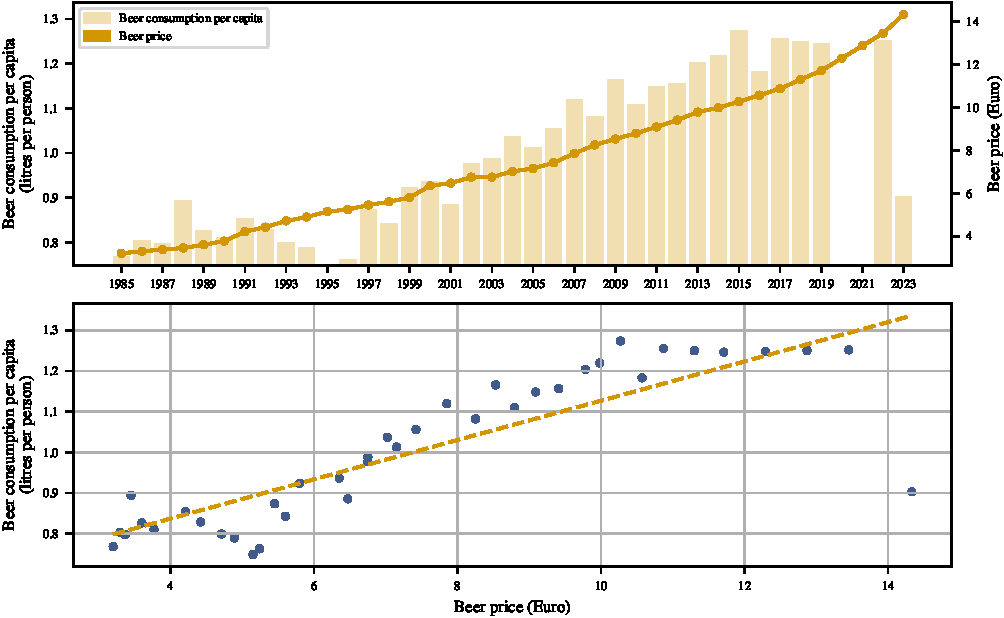
\includegraphics{fig/beer_consumption.pdf} % note no [width=\textwidth] needed
\caption{\textit{Top:} Beer price and beer consumption per capita between 1985 and 2023. \textit{Bottom:} Correlation between beer price and beer consumption per capita.}
\label{fig:beer_consumption}
\end{figure*}

\subsection*{3.5 Beer \& chicken price prediction}
The linear regression model utilized for beer price prediction exhibited impressive performance, forecasting a value of 14.29€ in 2023, which closely mirrors the observed price of 14.33€. The Gaussian Process Regression estimated the price to be 13.13€, accompanied by an uncertainty range of approximately ± 2.52.
Shifting the focus to chicken prices, the linear regression model projected a value of 13.82€ in 2023, deviating from the observed value of 16.49€. On the other hand, the Gaussian Process Regression provided a mean projected price of 13.08€, accompanied by an uncertainty range of approximately ± 1.96.
\begin{figure}[ht]
    % this figure made with plt.rcParams.update(bundles.icml2022(column="half”,usetex=False)) fig,ax = plt.subplots(nrows=1, ncols=1)
    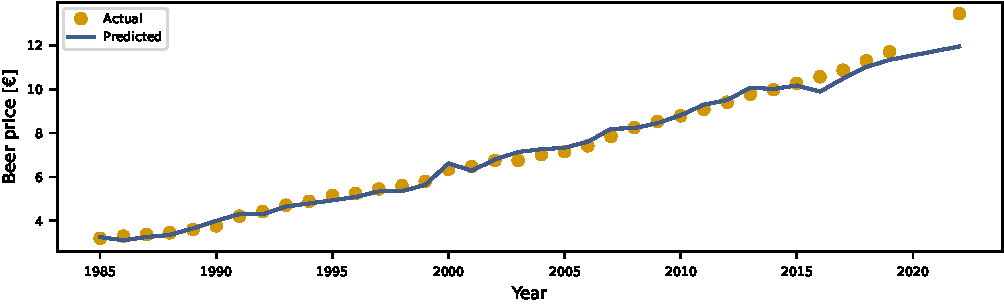
\includegraphics{fig/gaussian_beer_price_pred.pdf} 
    \caption{Beer Price Prediction from 1985 till 2023 using Gaussian process regression with an uncertainty level of one standard deviation for 2023.  }
    \label{figure_prediction}
\end{figure}




\section{Discussion \& Conclusion}\label{sec:conclusion}
The sudden drop in visitors in 2001 could potentially be explained by the 9/11 terrorist attacks that occurred a few weeks prior which almost resulted in the cancellation of the festival~\citep{9}. Perhaps surprisingly, visitor numbers were still very low during the first festival after the pandemic in 2022. This could be due to the public's remaining fears of contracting the virus in large crowds.\\
The weak correlation between mean precipitation at daytime and mean daily visitors indicates that precipitation does not have a great influence on festival attendance. This outcome is contrary to our expectations and can be attributed to various factors. One reason is the lack of daily visitor numbers, forcing us to rely on the mean over all days. However, examining the correlation of these means overlooks the variations in daily distributions, potentially leading to a weaker correlation. Nevertheless, this method still demonstrates that precipitation has only a minor effect on visitor numbers, with other factors, such as terrorist attacks, likely having a greater impact on festival attendance.\\
Rising beer prices do not deter beer consumption, as there is a positive correlation between beer price and per capita consumption. The Oktoberfest has grown in popularity since 1985 and now also attracts many international tourists. This could explain why people are willing to pay more for a "Maß" beer, particularly international tourists accustomed to similar prices in their home countries. Adjusting beer prices for inflation using the CPI further confirms the correlation's independence from inflation rates, as it isolates changes in real beer prices from general price increases in the economy. The 2023 Oktoberfest was the first to introduce free water fountains~\citep{8}, which could have contributed to the decrease in overall beer consumption we see that year. Interestingly, while beer consumption shows a positive correlation with price, chicken consumption trends in the opposite direction. However, the decrease in chicken consumption might have less to do with the increase in price, but rather with the rise in popularity of other foods.\\
The notable accuracy of the linear regression model, in contrast to the Gaussian process regression in predicting beer prices, may be attributed to the predominantly linear relationship of the beer prices. Consequently, for simplicity and computational efficiency, opting for the linear regression model would be a pragmatic choice for predicting beer prices.
On the other hand, both models perform poorly when predicting chicken prices. This could be attributed to the unusual increase in chicken prices around the year 2000, posing challenges for the models in capturing and adapting to such irregularities in the data.\\

As daily visitor numbers are unavailable, the monthly breakdown provides the most detailed information available. For our analysis, we assume that the majority of visitors to the Oktoberfest are included in the visitor numbers for September, especially the arrival figures, as the Oktoberfest starts in mid-September and most visitors are likely to arrive during this month. The fact that the Oktoberfest has an impact on visitor numbers beyond the city itself is indicated by the overall purple shading of the areas surrounding Munich. As Munich is already a popular tourist destination, smaller districts surrounding Munich benefit even more from the Oktoberfest, experiencing a higher percentage increase in visitor numbers. Interestingly, one district (Traunstein) is colored orange in many years, which means that there are fewer tourists than expected. There may be an event in Traunstein in August or October that drives up visitor numbers in that month.

\section*{Contribution Statement}
Jana Hoffmann analyzed the influence of precipitation on visitor numbers, Julia Graf investigated the influx of tourists to the surrounding area, Jessie Midgley looked at the correlation between consumption and prices, and Tithi Rakshit employed models to predict future prices. All authors contributed to the writing of the report.



\bibliography{bibliography}
\bibliographystyle{icml2023}

\end{document}


% This document was modified from the file originally made available by
% Pat Langley and Andrea Danyluk for ICML-2K. This version was created
% by Iain Murray in 2018, and modified by Alexandre Bouchard in
% 2019 and 2021 and by Csaba Szepesvari, Gang Niu and Sivan Sabato in 2022.
% Modified again in 2023 by Sivan Sabato and Jonathan Scarlett.
% Previous contributors include Dan Roy, Lise Getoor and Tobias
% Scheffer, which was slightly modified from the 2010 version by
% Thorsten Joachims & Johannes Fuernkranz, slightly modified from the
% 2009 version by Kiri Wagstaff and Sam Roweis's 2008 version, which is
% slightly modified from Prasad Tadepalli's 2007 version which is a
% lightly changed version of the previous year's version by Andrew
% Moore, which was in turn edited from those of Kristian Kersting and
% Codrina Lauth. Alex Smola contributed to the algorithmic style files.
